Dans le but de concrétiser cette approche, nous nous sommes inspirés du travail réalisé par \mbox{Guillaume} \mbox{Tisserant} et son équipe, présenté dans la partie~\ref{un_modele_de_representation_de_la_conscience} (page~\pageref{un_modele_de_representation_de_la_conscience}). La figure~\ref{modele_original} présente la structure du fonctionnement que pourrait avoir une conscience artificielle. Celle-ci conserve la plupart des caractéristiques d’une conscience humaine grâce à l'étude de nombreaux travaux comme ceux de Freud et de Laborit\footnote{Henri Laborit (1914--1995): Médecin chirurgien et neurobiologiste.}.

\begin{figure}[H] 
\centering
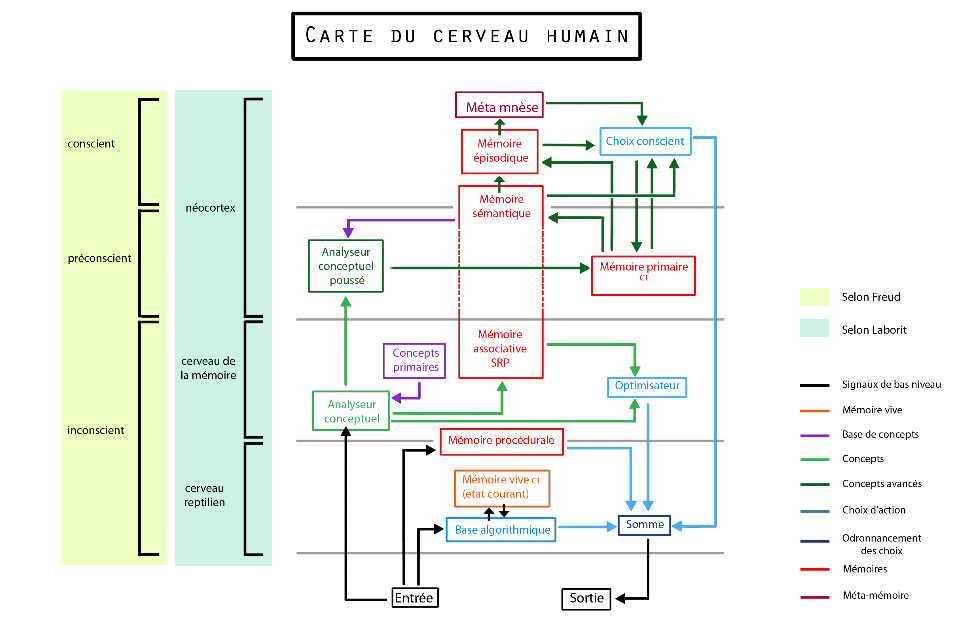
\includegraphics[width=\textwidth]{files/modele_original} 
\caption{Schéma du modèle de représentation de la conscience} 
\label{modele_original}
\end{figure}

Cette représentation peut être vu comme un empilement de couches : l'inconscient se situant au plus bas et le conscient au plus haut.

\subsection{L'inconscient}
L'inconscient est composé de deux niveaux : le cerveau reptilien le cerveau de
la mémoire.

\subsubsection{Le cerveau reptilien}

C'est la couche la plus basse du modèle.

\paragraph{Les entrées/sorties}
Les entrées permette au cerveau d'acquérir deux types d'informations :
\begin{itemize}
\item les percepts externes, émis par l'environnement et perçus par les cinq sens,
\item le percepts interne, comme les pulsions, etc. 
\end{itemize}

Les sorties assurent la transmission des informations produites par le cerveau au reste du corps.

\paragraph{La base algorithmique} Il s'agit d'une base simple assurant une réaction rapide à des entrées simples, en produisant des sorties simple. C'est cette partie qui stocke les réflexes innés présents chez les êtres vivants. 

\paragraph{La mémoire procédurale} Elle permet de construire des automatismes en fonction du vécu. Par exemple, selon un schéma essai échec, un bébé apprendra à marcher en utilisant sa mémoire procédurale.

\subsubsection{Le cerveau de la mémoire} Cette prochaine couche étant plus
complexe que la dernière, ici on trouve un analyseur conceptuel, une mémoire
associative et un optimisateur.
\subparagraph {L'analyseur conceptuel} compare des entrées en dur à une base de
données de concepts primaires (la faim, la soif, le plaisir, la fatigue, la joie, une odeur
nauséabonde, un bruit violent...).
\subparagraph {La mémoire associative} compare la réception de ces concepts
entre eux. Cela permet par exemple à un animal vivant dans un milieu contenant des prédateurs
bruyant d’associer le concept de danger au bruit que fait le prédateur.
\subparagraph {L’optimisateur} a pour vocation d’optimiser un concept qui peut
se traduire par le bien-être. Dans l’exemple précédent, il prend en compte que l’approche d’un
prédateur réduit le bien-être, et que le fait de courir peut éloigner le
prédateur, donc faire remonter le bien être. Il devra donc choisir l’action de
fuir.

\subsection{Le Néocortex : la préconscience et la conscience}
Les couches qui font partie du néocortex représentent la préconscience et la
conscience. C'est ici qu'on s'approche de la cognition humaine.
\subsubsection{Le préconscient} Cette couche consiste d'un analyseur
conceptuel sémantique et des mémoires primaire et sémantique.
\subparagraph{L'analyseur conceptuel sémantique} manipule des concepts un niveau
au dessus de ceux manipulés par l’analyseur conceptuel du cerveau de la mémoire. Il sert à
traduire les concepts primaires en concepts complexes stockés dans la mémoire
sémantique.
\subparagraph{La mémoire sémantique} contient donc une base de
données de concepts avancés, construite sous forme de treillis reliant les concepts ensemble.
\subparagraph{La mémoire primaire} contient un très petit nombre de concepts
sémantiques. Elle contient les choses auxquels auquel une conscience est en
train de penser. Elle peut être remplie par l’analyseur conceptuel sémantique qui lui envoie les
concepts se trouvant dans l’environnement, ou directement par la réflexion
consciente qui choisit d’y poser un concept pour réfléchir dessus.
\subparagraph{La gestion de la mémoire sémantique} est complexe : les concepts
en mémoire primaire sont copiés en mémoire sémantique instantanément. Tout ce qui est en
mémoire primaire y arrive, mais les choses sont aussi oubliées petit à petit.
Plus elles restent ou repassent en mémoire primaire, moins elles disparaissent
de la mémoire sémantique.
\subsubsection{Le conscient} Dans cette couche se trouvent les modules les plus
avancés du modèle : la mémoire épisodique, la méta Mnèse  et le choix conscient.
\subparagraph{La mémoire épisodique} est une mémoire des situations. Elle sert à
se remémorer des situations et des émotions vécus sous formes de concepts sémantiques. Les
concepts stockés viennent à la fois des percepts mais aussi de l’état interne de
la personne au moment de l’événement. Elle gère la persistance de la même
manière que la mémoire sémantique.
\subparagraph{La méta Mnèse} est la mémoire de la mémoire. Son rôle est de stocker la
façon dont les éléments se sont enchaînés dans la mémoire épisodique.
\subparagraph{Le choix conscient} (ou réflexion consciente) ressemble à l'optimisateur,
mais maniant des concepts de plus hauts niveaux, et de natures différentes. Grâce à
la méta Mnèse, il peut utiliser des séries de situations, et même imaginer des
situations passées, présentes ou futures pour prendre des décisions. Il peut
ainsi comparer des situations imaginaires et choisir celle vers laquelle il a
envie de tendre. Il peut aussi réfléchir sur des concepts abstraits, comme sur
ses réflexions passés. Il peut analyser son propre fonctionnement à partir du
moment où il arrive à le retranscrire sous forme de concepts.

\section{Synthèse}
L’objet représenté par \textbf{Somme} dans la couche du cerveau reptilien
est une simplification du schéma retour. Il représente la transformation de tous les
signaux en signaux de bas niveaux, et gère la somme des signaux pour choisir
lesquels inhiber et lesquels renvoyer en sortie. Son fonctionnement nécessite
d’arriver à combiner les signaux entre eux. Par exemple, si une personne choisit
de fumer dans le choix conscient, il doit récupérer la façon d’allumer un
briquet dans la mémoire procédurale.
